% mnras_template.tex
%
% LaTeX template for creating an MNRAS paper
%
% v3.0 released 14 May 2015
% (version numbers match those of mnras.cls)
%
% Copyright (C) Royal Astronomical Society 2015
% Authors:
% Keith T. Smith (Royal Astronomical Society)

% Change log
%
% v3.0 May 2015
%    Renamed to match the new package name
%    Version number matches mnras.cls
%    A few minor tweaks to wording
% v1.0 September 2013
%    Beta testing only - never publicly released
%    First version: a simple (ish) template for creating an MNRAS paper

%%%%%%%%%%%%%%%%%%%%%%%%%%%%%%%%%%%%%%%%%%%%%%%%%%
% Basic setup. Most papers should leave these options alone.
\documentclass[fleqn,usenatbib]{mnras}

% MNRAS is set in Times font. If you don't have this installed (most LaTeX
% installations will be fine) or prefer the old Computer Modern fonts, comment
% out the following line
\usepackage{newtxtext,newtxmath}
% Depending on your LaTeX fonts installation, you might get better results with one of these:
%\usepackage{mathptmx}
%\usepackage{txfonts}

% Use vector fonts, so it zooms properly in on-screen viewing software
% Don't change these lines unless you know what you are doing
\usepackage[T1]{fontenc}
\usepackage{ae,aecompl}


%%%%% AUTHORS - PLACE YOUR OWN PACKAGES HERE %%%%%

% Only include extra packages if you really need them. Common packages are:
\usepackage{graphicx} % Including figure files
\usepackage{amsmath} % Advanced maths commands
\usepackage{amssymb} % Extra maths symbols
\usepackage{xcolor} % Colour text for draft

%%%%%%%%%%%%%%%%%%%%%%%%%%%%%%%%%%%%%%%%%%%%%%%%%%

%%%%% AUTHORS - PLACE YOUR OWN COMMANDS HERE %%%%%

% Please keep new commands to a minimum, and use \newcommand not \def to avoid
% overwriting existing commands. Example:
%\newcommand{\pcm}{\,cm$^{-2}$} % per cm-squared

% Use bold font for vectors
\let\vec\mathbf

%%%%%%%%%%%%%%%%%%%%%%%%%%%%%%%%%%%%%%%%%%%%%%%%%%

%%%%%%%%%%%%%%%%%%% TITLE PAGE %%%%%%%%%%%%%%%%%%%

% Title of the paper, and the short title which is used in the headers.
% Keep the title short and informative.
\title[Hybrid multigrain]{Hybrid multigrain: A smoothed particle hydrodynamics
algorithm for small and large dust grains}

% The list of authors, and the short list which is used in the headers.
% If you need two or more lines of authors, add an extra line using \newauthor
\author[Mentiplay, Price, Laibe, \& Pinte]{%
   \parbox{\textwidth}{%
      Daniel Mentiplay\(^{1}\)\thanks{daniel.mentiplay@monash.edu},
      Daniel J. Price\(^{1}\),
      Guillaume Laibe\(^{2}\),
      Christophe Pinte\(^{1,3}\)}\\
   \(^{1}\)Monash Centre for Astrophysics (MoCA) and School of Physics and
   Astronomy, Monash University, Clayton Vic 3800, Australia \\
   \(^{2}\)Lyon, France \\
   \(^{3}\)Univ. Grenoble Alpes, CNRS, IPAG, F-38000 Grenoble, France}

% These dates will be filled out by the publisher
\date{Accepted XXX. Received YYY; in original form ZZZ}

% Enter the current year, for the copyright statements etc.
\pubyear{2020}

% Don't change these lines
\begin{document}
\label{firstpage}
\pagerange{\pageref{firstpage}--\pageref{lastpage}}
\maketitle

% Abstract of the paper
\begin{abstract}
\end{abstract}

% Select between one and six entries from the list of approved keywords.
% Don't make up new ones.
\begin{keywords}
keyword1 -- keyword2 -- keyword3
\end{keywords}

%%%%%%%%%%%%%%%%%%%%%%%%%%%%%%%%%%%%%%%%%%%%%%%%%%

%%%%%%%%%%%%%%%%% BODY OF PAPER %%%%%%%%%%%%%%%%%%

\section{Introduction}

\textcolor{red}{
\begin{itemize}
   \item Dust-gas modeling in astrophysical fluids.
   \item Single grain size vs multiple dust species.
   \item \citet{Haworth2016PASA...33...53H}---grand challenges in protoplanetary disc
      modeling.
   \item Applications: protoplanetary discs, molecular clouds.
   \item Phantom dust methods---\citet{Price2018PASA...35...31P}.
   \item Phantom 1-fluid multigrain---\citet{Hutchison2018MNRAS.476.2186H}.
\end{itemize}
}

\section{Methods}

\subsection{Continuum equations for multiple dust species}

The equations of conservation of momentum for a multiple species dust and gas
mixture are given by
%
\begin{align}
   \rho_g \frac{d \vec{v}_g}{dt} &= - \nabla P + \sum_i K_i \left(\vec{v}_{d_i}
                                    - \vec{v}_{g}\right), \\
   \rho_{d_i} \frac{d \vec{v}_{d_i}}{dt} &= - K_i \left(\vec{v}_{d_i}
                                                       - \vec{v}_{g}\right),
\end{align}
%

\subsection{SPH with multiple dust species}

\subsection{Stopping time}

\textcolor{red}{
\begin{itemize}
   \item Discuss large grains vs small grains, strong vs weak coupling, and
      terminal velocity approximation.
\end{itemize}
}
For a single dust species the stopping time, i.e.\ the drag timescale, \(t_s\)
is
%
\begin{align}
   t_s = \frac{\rho_g \rho_d}{K (\rho_g + \rho_d)},
\end{align}
%
where \(K\) is the drag coefficient for the single species. We assume spherical
grains of size \(s\) with a uniform material density, \(\rho_m\). In the linear
Epstein regime \citep{Epstein1924PhRv...23..710E} the drag coefficient \(K\) is
%
\begin{align}
   K = \frac{\rho_g \rho_d}{\rho_m s} \sqrt{\frac{8}{\pi\gamma}} c_s.
\end{align}
%
As discussed in \citet{Hutchison2018MNRAS.476.2186H}, a straightforward
generalisation of the stopping time for multiple dust species is not available.
Each dust species is separately coupled to the gas by the drag force. However,
the dust species are indirectly coupled to each other via backreaction, i.e.\
conservation of momentum. For convenience, we define an effective material
density, \(\rho_{\mathrm{eff}}\), given by
%
\begin{align}
   \rho_{\mathrm{eff}} = \rho_m \sqrt{\pi\gamma/8}.
\end{align}
%
The drag coefficient of each dust species, \(K_i\), is now
%
\begin{align}
   K_i = \frac{\rho_g \rho_{d_i} c_s}{\rho_{\mathrm{eff}} s_i},
\end{align}
%
and we can define a time scale, \(t_{s_i}\), as
%
\begin{align}
   t_{s_i} = \frac{\rho}{K_i},
\end{align}
%
where \(\rho = \rho_g + \sum_i \rho_{d_i}\) is the total density of the gas and
all dust species.

\subsection{Time stepping}

\section{Numerical tests}

\subsection{Dusty-box}

\begin{figure*}
   \begin{center}
      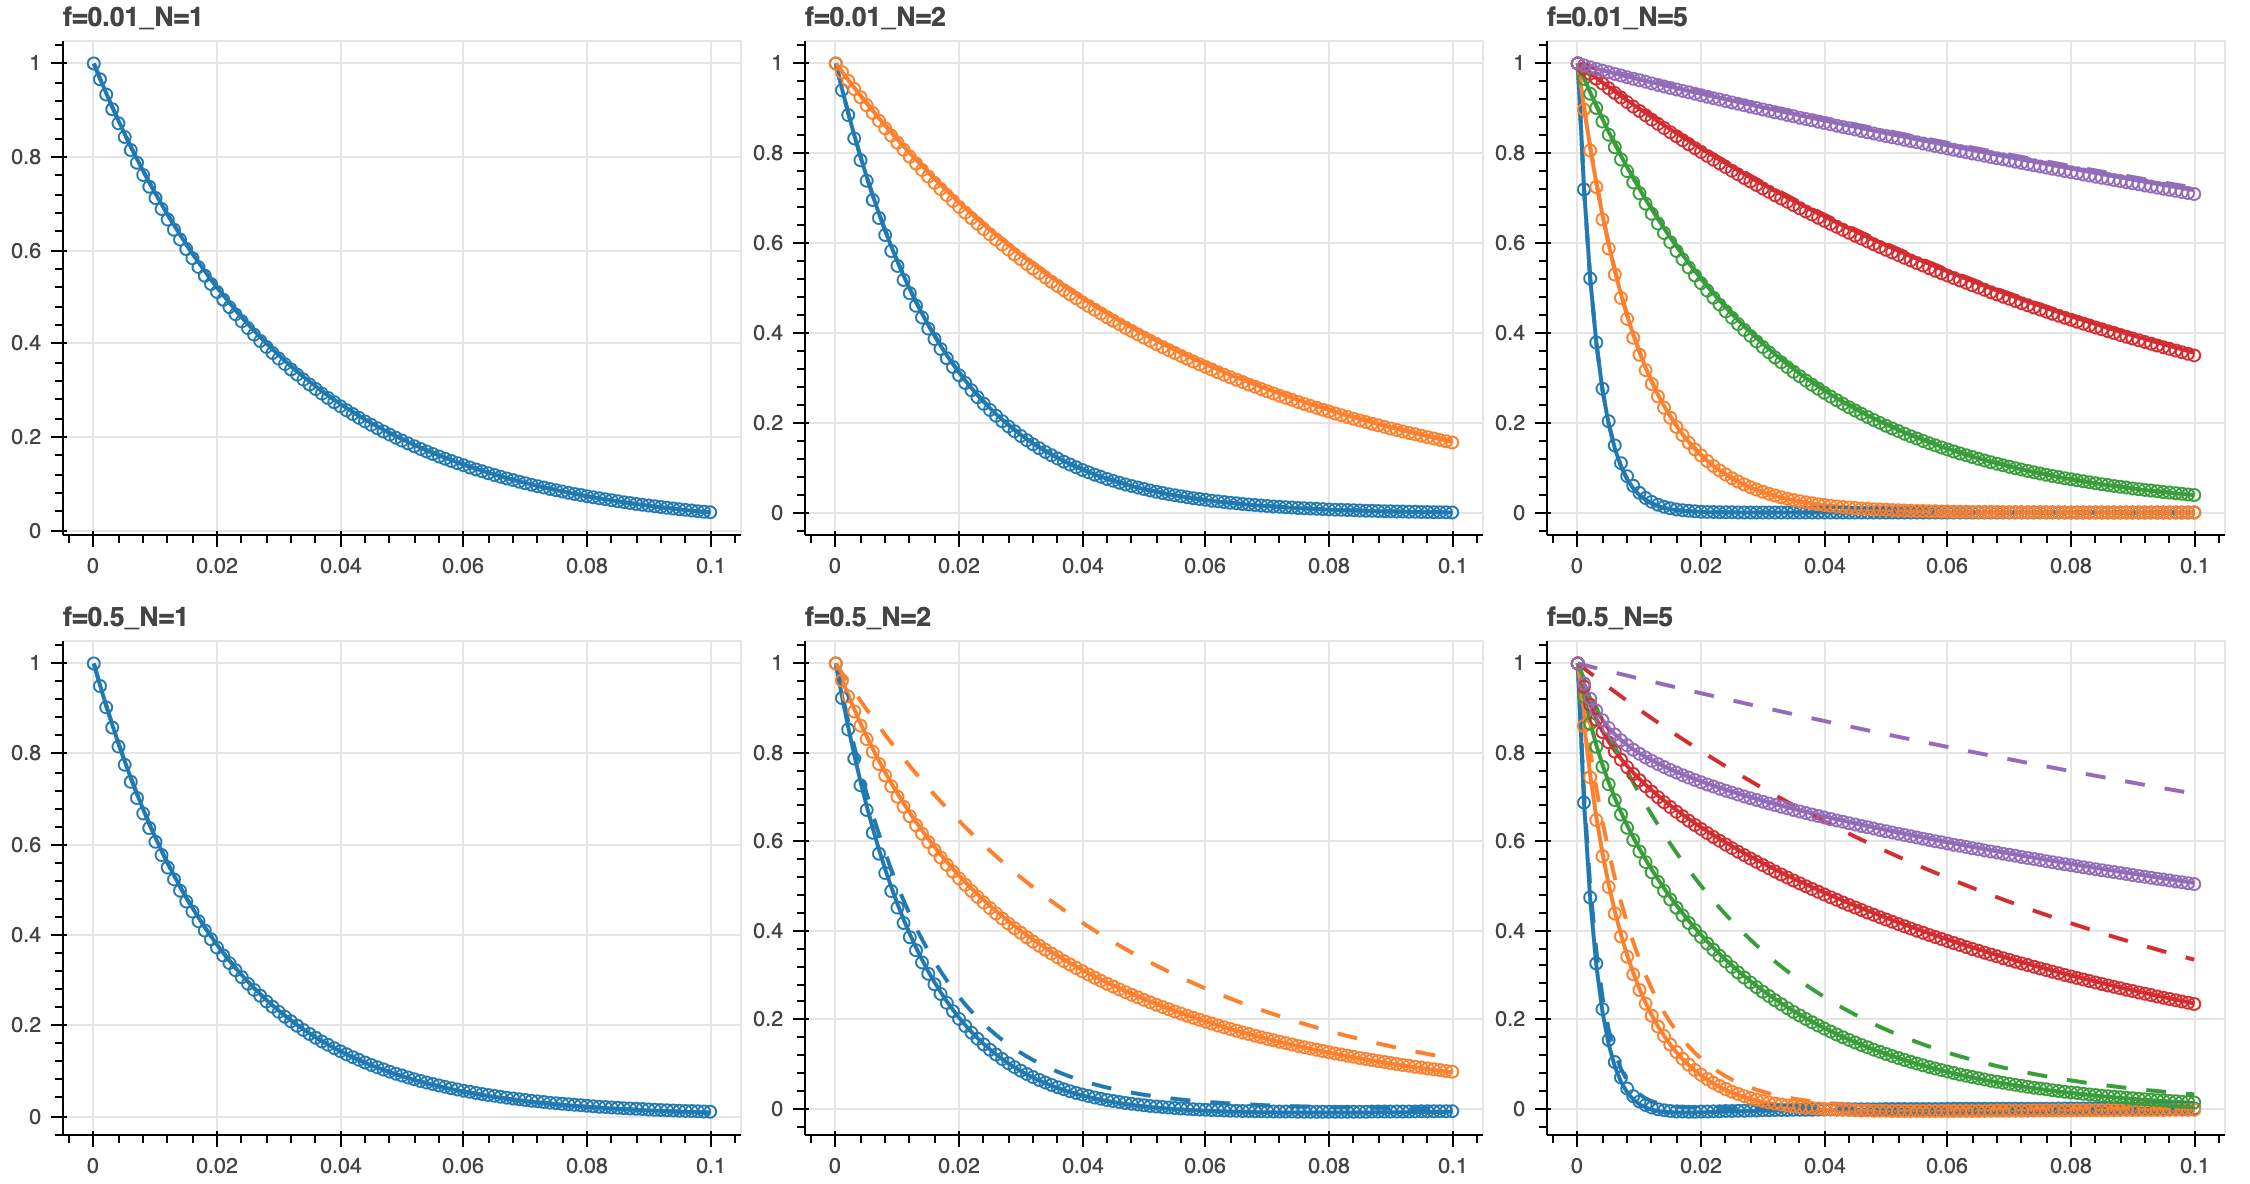
\includegraphics[width=\textwidth]{figs/dustybox.png}
      \caption{Dusty-box numerical test showing the differential velocity
         between the dust and gas. The total dust-to-gas ratio is 0.01 (top row)
         and 0.5 (bottom row). From left to right: the number of dust species is
         1, 2, 5. The open circles represent the results from the Phantom
         simulation. The solid and dashed lines represent the analytical
         solution with and without, respectively, taking back reaction into
         account.\label{fig:dustybox}}
   \end{center}
\end{figure*}

We performed the multigrain version of the dusty-box test described in
\citet{Laibe2011MNRAS.418.1491L}. The dusty-box involves setting up a periodic
box of uniform density gas and dust with an initial differential velocity
between the gas and dust. In this test the equation of motion simplifies to
%
\begin{align}
   \frac{\partial \Delta \vec{V}}{\partial t} = - \Omega_n \Delta \vec{V},
\end{align}
%
where \(\Delta \vec{V}\) is the differential velocity vector, and \(\Omega_n\)
is the drag matrix given in Eq.~64 of \citet{Laibe2014MNRAS.444.1940L}.
Dusty-box is a test of the exchange of momentum between gas and dust species via
the drag force. The original dusty-box test was for a single grain size. We ran
the multigrain version described in \citet{Laibe2014MNRAS.444.1940L} in the
linear Epstein drag regime \citep{Epstein1924PhRv...23..710E}. We chose the
physical Epstein drag prescription in Phantom.

We performed six tests in two sets of three. The first set had a total
dust-to-gas ratio of 0.01, and the second set 0.5. The tests within each set had
1, 2, and 5 dust species, respectively, with grain sizes: 1.0 cm for the 1 dust
species test; 0.562 cm and 1.78 cm for the 2 species test; and 0.1 cm, 0.316 cm,
1.0 cm, 3.16 cm, and 10.0 cm for the 5 species test. Each test had equal mass in
each grain size bin. The gas is initially motionless, and each dust species has
uniform velocity in the positive x-direction.

For each test problem, we set up each of the gas and dust fluids on a
close-packed lattice, such that there were 32 gas particles in the direction of
motion, and, for each dust species, 16 dust particles. We set the gas density to
\(10^{-13}\)~g~cm\({}^{-3}\), with dust density varying per test problem. We set
the dust grain density to \(0.5 \times 10^{-14}\)~g~cm\({}^{-3}\).

Figure~\ref{fig:dustybox} shows the time evolution of the mean velocity
differential between the gas and each dust species, compared with analytical
solutions. The dashed lines represent the analytical solution without
backreaction from the dust on the gas. The solid lines represent the analytical
solution including backreaction. For low dust-to-gas ratio (0.01) both
analytical solutions give the same decay of differential velocity, with which
the Phantom simulation agrees. For a larger dust-to-gas ratio (0.5) the
analytical solutions diverge, and the Phantom simulation data follows the
backreaction-inclusive solution. For large dust-to-gas ratio we see that the
smaller grains (0.1 cm and 0.316 cm) rapidly slow and the differential velocity
reverses sign. I.e. the small grains slow to the gas velocity; then, as the
larger grains speed up the gas via drag, the gas drags the small grains along
with it. This shows that the behaviour of multiple dust species for large
dust-to-gas ratios requires taking back reaction into consideration to capture
the physics of dust drag accurately
\citep{Gonzalez2017MNRAS.467.1984G,Dipierro2018MNRAS.479.4187D}.

\subsection{Dusty-wave}

\begin{figure*}
   \begin{center}
      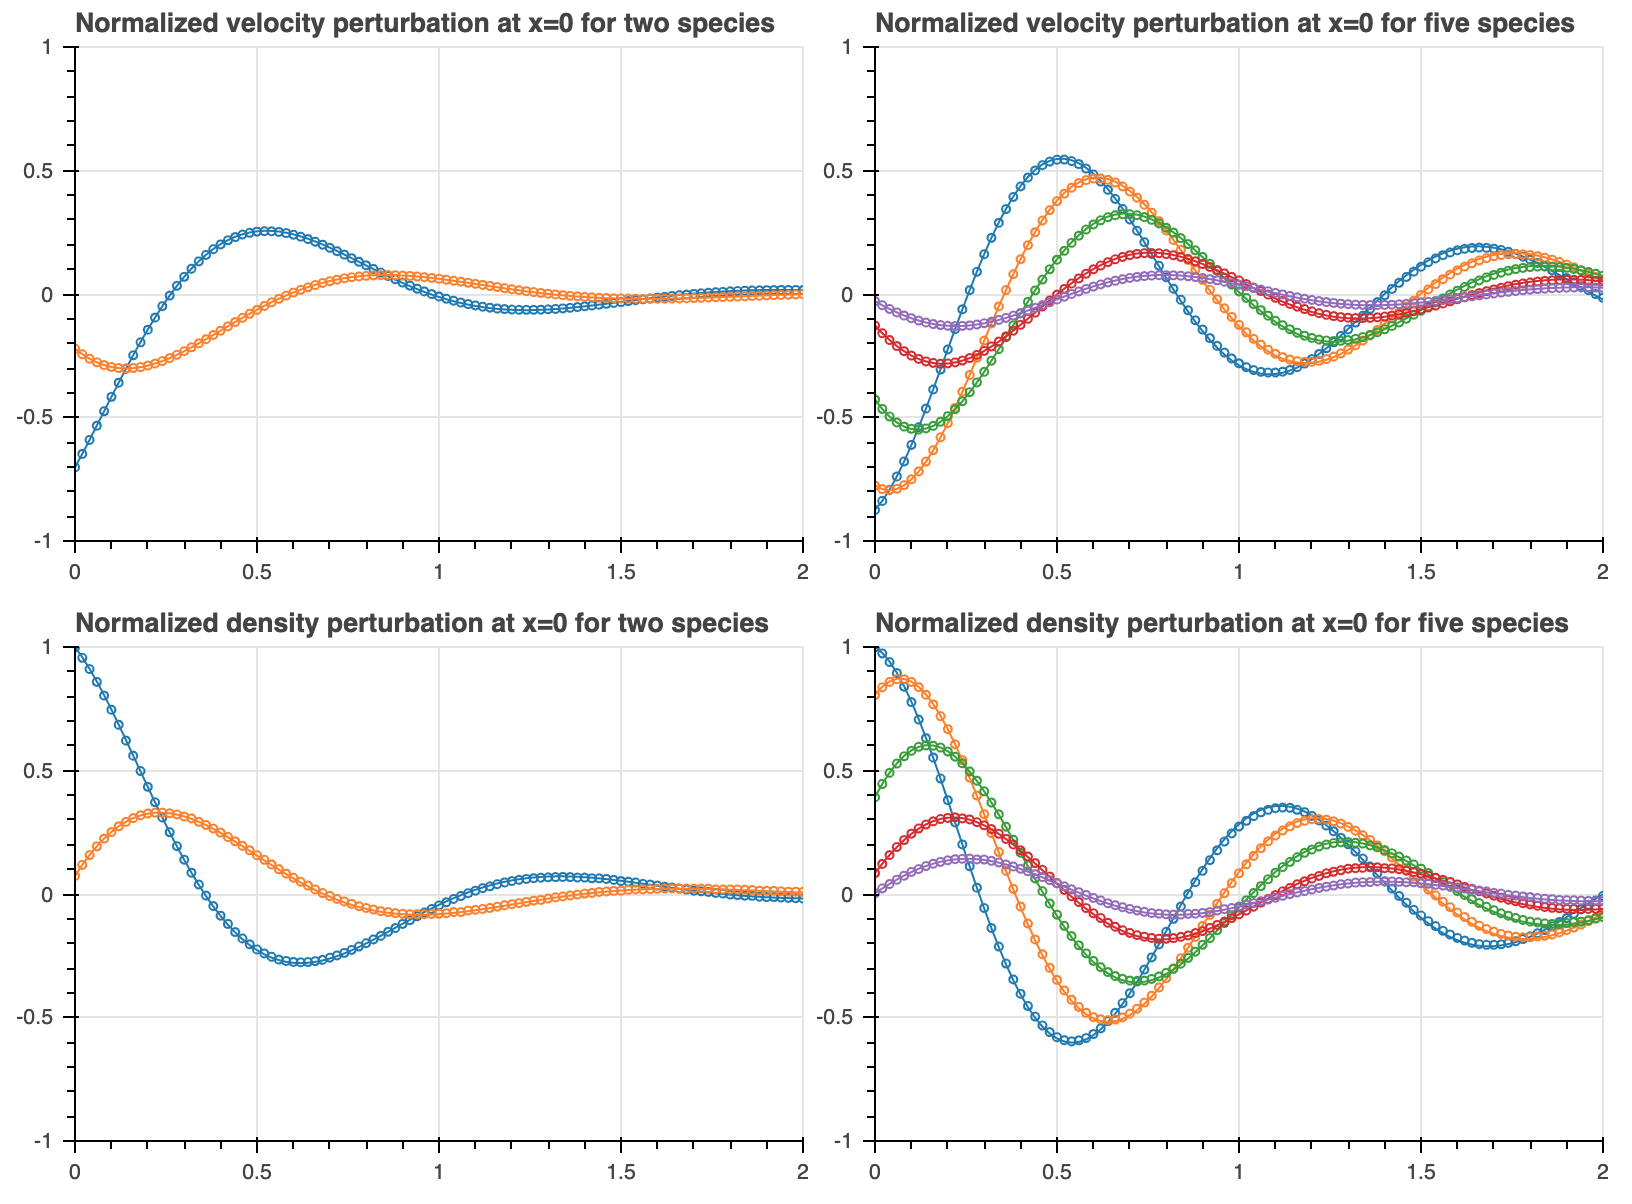
\includegraphics[width=\textwidth]{figs/dustywave.png}
      \caption{Dusty-wave numerical test showing the velocity perturbation (top)
         and the density perturbation (bottom) at \(x = 0\), for gas with one
         dust species (left) and gas with four dust species (right). The open
         circles represent the Phantom simulation, and the solid line represents
         the analytical solution from
         \citet{Benitez-Llambay2019ApJS..241...25B}.\label{fig:dustywave}}
   \end{center}
\end{figure*}

We performed the multigrain version of the dusty-wave test described in
\citet{Laibe2011MNRAS.418.1491L}. This is a test of the dust-gas drag coupling
in the context of a damped sound wave. The dust is a pressureless fluid and
cannot support sound waves. However, the gas can support sounds waves and drags
the dust. This leads to damping. For the particular setup we followed
\citet{Benitez-Llambay2019ApJS..241...25B}.

\subsection{Dusty-shock}

\subsection{Other tests?}

\begin{itemize}
   \item Radial drift.
   \item Settling.
\end{itemize}

\section{Application}

\subsection{Circumbinary disc}

Do a comparison between multiple single grain calculations vs one multigrain
calculation focussing on dust trapping in a circumbinary disc. For example, in
HD~142527. The figure would show a phase difference between the dust (or gas)
distribution comparing the single-grain vs multigrain calculation.

\section{Discussion}

\section{Conclusions}

\section*{Acknowledgements}


%%%%%%%%%%%%%%%%%%%%%%%%%%%%%%%%%%%%%%%%%%%%%%%%%%

%%%%%%%%%%%%%%%%%%%% REFERENCES %%%%%%%%%%%%%%%%%%

% The best way to enter references is to use BibTeX:

\bibliographystyle{mnras}
\bibliography{multigrain-paper}


%%%%%%%%%%%%%%%%%%%%%%%%%%%%%%%%%%%%%%%%%%%%%%%%%%

%%%%%%%%%%%%%%%%% APPENDICES %%%%%%%%%%%%%%%%%%%%%

% \appendix

% \section{Some extra material}


%%%%%%%%%%%%%%%%%%%%%%%%%%%%%%%%%%%%%%%%%%%%%%%%%%


% Don't change these lines
\bsp % typesetting comment
\label{lastpage}
\end{document}
% End of mnras_template.tex
